\begin{itshape}
En mathématiques, \emph{l'ensemble de Mandelbrot} est une fractale définie comme l'ensemble des points $c \in \mathbb{C}$ pour lesquels la suite de nombres complexes définie par récurrence par :
\begin{equation}\label{mandelbrot}
\left\{
\begin{array}{r c l}
z_0 &=& 0\\
z_{n+1} &=& z^2_n+c
\end{array}
\right.
\end{equation}
est bornée.
\setlength{\parskip}{3 mm}

\emph{L'ensemble de Mandelbrot} (notée aussi $\mathcal{M}$) a été découvert par Gaston \textsc{Julia} et Pierre \textsc{Fatou} avant la Première Guerre mondiale. Sa définition et son nom actuel sont dus à Adrien \textsc{Douady}, en hommage aux représentations qu'en a réalisées Benoît \textsc{Mandelbrot} dans les années 1980. Cet ensemble permet d'indicer \emph{les ensembles de Julia} : à chaque point du plan complexe correspond un ensemble de Julia différent. Les points de \emph{l'ensemble de Mandelbrot} correspondent précisément aux \emph{ensembles de Julia} connexes, et ceux en dehors correspondent aux \emph{ensembles de Julia} non connexes. Cet ensemble est donc intimement lié à \emph{l'ensemble de Julia}, ils produisent d'ailleurs des formes similairement complexes.
\setlength{\parskip}{2 mm}

Les images de \emph{l'ensemble de Mandelbrot} sont réalisées en parcourant les nombres complexes sur une région carrée du plan complexe. Les point de cette région du plan complexe se divisent en deux catégories : ceux qui génèrent une suite non bornée et ceux qui génèrent une suite bornée avec la relation de récurrence (\ref{mandelbrot}). On considère la partie réelle et imaginaire de chaque nombre complexe comme des coordonnées. Si le pixel converge, alors il est coloré en noir. Sinon, on le colorie selon sa rapidité de divergence.
\end{itshape}

\begin{figure}\label{Ensemble de Mandelbrot en noir}
\centering
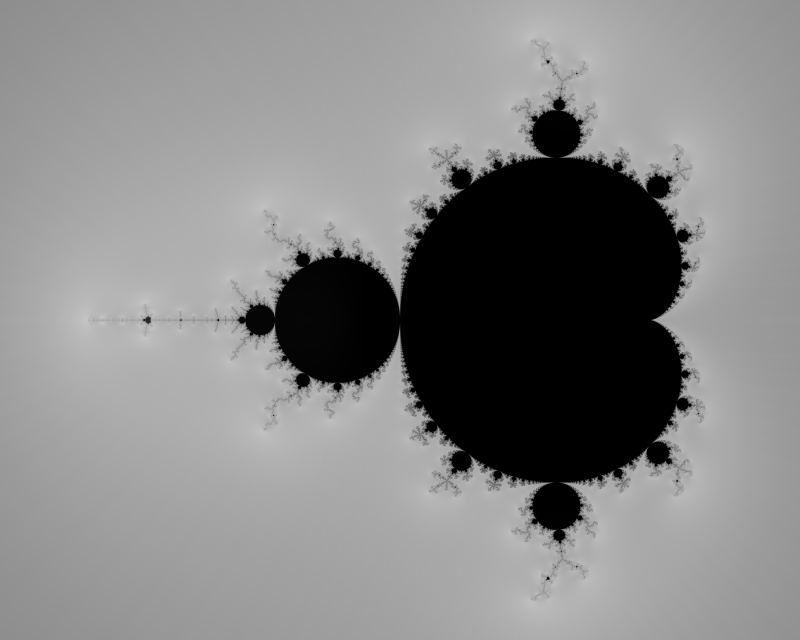
\includegraphics[scale=0.1]{images/Ensemble de Mandelbrot en noir.png}
\caption{Ensemble de Mandelbrot en noir}
\end{figure}